%
% File acl2017.tex
%
%% Based on the style files for ACL-2015, with some improvements
%%  taken from the NAACL-2016 style
%% Based on the style files for ACL-2014, which were, in turn,
%% based on ACL-2013, ACL-2012, ACL-2011, ACL-2010, ACL-IJCNLP-2009,
%% EACL-2009, IJCNLP-2008...
%% Based on the style files for EACL 2006 by 
%%e.agirre@ehu.es or Sergi.Balari@uab.es
%% and that of ACL 08 by Joakim Nivre and Noah Smith

\documentclass[11pt,a4paper]{article}
\usepackage[hyperref]{acl2017}
\usepackage{times}
\usepackage{latexsym}


\usepackage{url}

\aclfinalcopy % Uncomment this line for the final submission
%\def\aclpaperid{***} %  Enter the acl Paper ID here

%\setlength\titlebox{5cm}
% You can expand the titlebox if you need extra space
% to show all the authors. Please do not make the titlebox
% smaller than 5cm (the original size); we will check this
% in the camera-ready version and ask you to change it back.

\newcommand\BibTeX{B{\sc ib}\TeX}
\usepackage{graphicx}
\usepackage{float}
\usepackage{placeins}
\usepackage{subcaption}
\usepackage{cleveref}
\usepackage{listings}
\usepackage{graphicx}
\usepackage{enumitem}
\usepackage{amsmath}
\usepackage{amssymb}

\usepackage{mathtools}
\DeclarePairedDelimiter{\ceil}{\lceil}{\rceil}

\newcommand{\acomment}[1]{{\bf{\color{blue}{{[Aman: #1]}}}}}
\newcommand{\bigo}[1]{\ensuremath{\mathcal{O} (#1)}}
\newcommand{\fullref}[1]{\hyperref[{#1}]{\autoref*{#1} - \nameref*{#1}}} % One single link
\newcommand{\figref}[1]{\hyperref[{#1}]{\autoref*{#1}}} % One single link


\title{Debunking Neural Essay Scoring}

\author{Aman Agrawal \\
  IIT Delhi \\
  {\tt cs1150210@iitd.ac.in} \\\And
  Suyash Agrawal \\
  IIT Delhi \\
  {\tt cs1150262@iitd.ac.in} \\}

\date{}

\begin{document}
\maketitle
\begin{abstract}
  Automated essay scoring systems(AES) are used in evaluating and scoring student essays written based on a given prompt. Recent advances in Deep Learning and Natural Language Processing have produced state of art results in this task. These systems are approaching human level performance according to the evaluation metrics, but their qualitative performance in actual scenarios is not yet explored. In this paper we explore and analyze how these systems perform in real life scenarios as compared to other non-neural models. We also explore some ways to overcome these shortcomings.
\end{abstract}

\section{Introduction}


Essay writing is one of the most popular ways to assess the skill of a student. Educational Testing Service (ETS)\cite{ets} uses essay scoring to assess the writing skill of students, but due to large number of students participating in these exams, it becomes very time consuming.
Automated essay scoring systems (AES) aims to automate the process of scoring essays. This is usually addressed as a supervised regression problem and the performance is judged by comparing the scores to a manually curated dataset of scored essays.
Recently, a lot of neural methods were proposed for this task and these have shown to give near human level performance in it. They seem to outperform the traditional feature based non-neural models like Enhanced AI Scoring Engine (EASE) \cite{ease}.
In this paper we explore the performance of deep-learning based systems on real life scenarios. We try to see compare their performance to traditional non-neural models in a qualitative sense and analyze the issues caused by them.


% Essay writing is usually a part of the student assessment  process. Several  organizations, such as Educational Testing Service (ETS)\cite{ets}, evaluate the writing skills of students in their examinations. Because of the large number of students participating in these exams, grading all essays is very time-consuming. 
% Thus, automated essay scoring systems(AES) are used in evaluating and scoring student essays written based on a given prompt. The performance of these systems is assessed by comparing their scores assigned to a set of essays to human-assigned gold-standard scores.
% Since the output of AES systems is usually a real valued number, the task is often addressed as a supervised machine learning task.
% Recently, there is a lot of development of deep neural models for the task of automated essay scoring.
% These models have shown to out perform the traditional models based on hand crafted features and currently have the state of art performance in this task. The current state of art model that we presently know of is from Taghipour et al. \cite{nea} and the state of art non-neural model is Enhanced AI Scoring Engine (EASE) \cite{ease}.
% In this paper we explore the performance of deep-learning based systems on real life scenarios. We try to see if their performance is actually better than traditional non-neural based models in a qualitative sense and analyze the issues that these systems can cause.

  % The rest of this paper is organized as follows. Section 2 gives an overview of related work in the literature. Section 3 describes the  details of our experiments, and present and discuss the results of our experimental evaluation in Section 4. Finally, we suggest some ways to improve the models in Section 5 and conclude the paper in Section 6.


\section{Related Work}

Currently, there are a lot of essay scoring systems like E-rater \cite{attali2004automated}. The non-neural essay scorer that we use in our analysis is Enhanced AI Scoring Engine (EASE) \cite{ease}
by edx, which came 3rd in the kaggle competition named \textit{Automated Student Assessment Prize (ASAP)} sponsored by Hewlett Foundation.\\
Traditionally, the models used various kinds of hand engineered features like: grammaticality \cite{attali2004automated}, essay length \cite{chen2013automated}, text coherence and organization of ideas\cite{chen2013automated} etc.\\

Recently, due to surge in the area of deep-learning, a lot of neural models have been proposed which claim to beat the human level performance on evaluation metrics. These models accept an essay text as input and learn the features automatically. Various architectures using LSTMs \cite{taghipour2016neural}, CNNs\cite{dong2016automatic} etc. have been proposed for automatically learning the features. 

% There exist many automated essay scoring systems \cite{shermis2013handbook} and some of them are being used in high-stakes assessments. E-rater \cite{attali2004automated} and E-rater \cite{attali2004automated} are two notable examples of AES systems. In 2012, a competition on automated essay scoring called \textit{Automated Student Assessment Prize (ASAP)} was organized by Kaggle and sponsored by the Hewlett Foundation. A comprehensive comparison of AES systems was made in the ASAP competition. Many AES systems have been developed to date, and most of them have been built with hand-crafted features and supervised machine learning algorithms. Researchers have devoted a substantial amount of effort to design effective features for automated essay scoring. These features can be as simple as essay length \cite{chen2013automated} or more complicated such as lexical complexity, grammaticality of a text \cite{attali2004automated}, or syntactic features \cite{chen2013automated}. Readability features \cite{zesch2015task} have also been proposed in the literature as another source of information. Moreover, text coherence has also been exploited to assess the flow of information and argumentation of an essay \cite{chen2013automated}. A detailed overview of the features used in AES systems can be found in \cite{zesch2015task}. 

% Recently due to surge in deep-learning, a lot of neural models have been proposed which claim to beat the human level performance on evaluation metrics. Unlike traditional systems these systems, accepts an essay text as input directly and learns the features automatically from the data. A lot of models with varying architectures have been developed in the recent years. Some of them use a long short-term memory network (LSTM) \cite{taghipour2016neural}, while others use a convolutional neural networks (CNN) \cite{dong2016automatic} for the effect of automatically learning features. Some of them also use an augmented method to learn word embeddings \cite{alikaniotis2016automatic}. 

We have tried to analyze these models over various qualitative metrics on which a human scorer would have graded the essays. We consider the length of the essay, grammatical and spelling mistakes, and the flow of ideas and organization of essay. Along with this, we also try to test if any of these models recognize deviation from the specifed topic. We finally suggest some ways to improve the performance of model on these qualitative metrics.



\section{Models}\label{sec:models}

\subsection{Neural Model}

The present state of the art neural model is from \cite{taghipour2016neural}. They use a simple a LSTM based model, where the output of each LSTM unit is averaged over time, to get a representation of the essay. Finally, they use a linear layer with sigmoid activation which maps its input vector generated by the mean-over-time layer to a scalar value and limits the possible scores to the range of $(0, 1)$.

\subsection{Non-Neural Model}
This model numerous features to create a vector representation of the essay. The features are chosen to take essay length, spelling mistakes, grammatical correctness and some of content-based features in account thus giving potential to the model to perform well in scoring task.


\section{Experiments}

\subsection{Setup}
The dataset that we have used in our experiments is the same dataset used in the ASAP competition run by Kaggle. We use quadratic weighted Kappa as a quantitative evaluation metric. We trained both the state of the art models described in \cref{sec:models} using the code released by the authors. Same hyper-parameters were used as reported in respective papers in order to reproduce the results stated in the papers.

The dataset contains essay from eight different prompts. Since the test data is not publicly available, the model was trained on 64\% of the data and tested on the remaining 20\%. The remaining 16\% was used to tune hyper-parameters and select the best model.
All of our analysis stated below has been done using the test dataset.

\subsection{Effect of Length}

We tried to analyze the effect of the length of the essay on the prediction of the models. Typically, low scoring essays have low scores and this can be seen from \cref{fig:length_plot}. Let, $\mu_l$ denote the mean length of the essays in the test set and $\sigma_l$ denote the standard deviation of the lengths. We selected essays from each prompt that had length less than $\mu_l - 2\sigma_l$ and appended the same essay till the point where the length of the essay exceeded $\mu_l + 2\sigma_l$. The mean score of these essays before and after increasing length were calculated and the percentage increase in the score was reported. \cref{length} shows that the average increase in the predicted score of the essay is $100.58\%$ while for some test sets the increase in the score was close to $235.53\%$. 

\begin{figure*}
  \centering             
  \begin{subfigure}[ht]{0.475\textwidth}
      \centering
      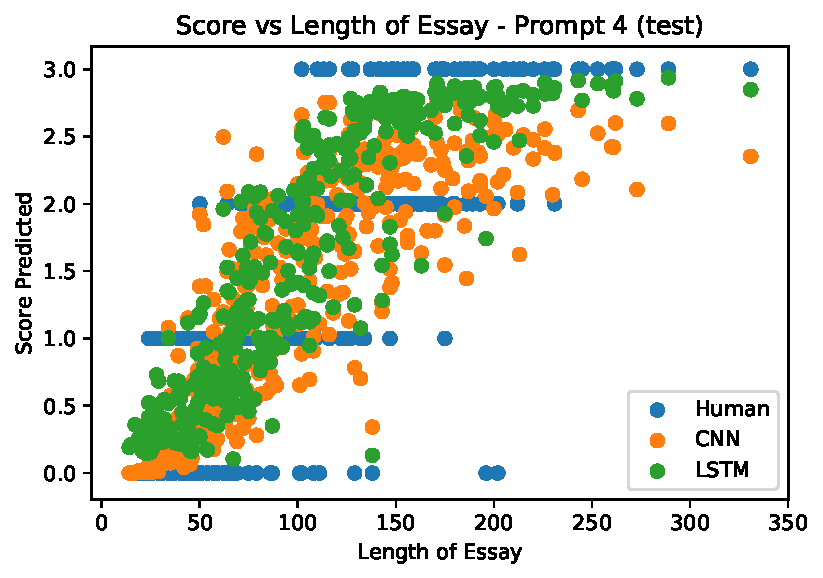
\includegraphics[width=\textwidth,ext=pdf]{{../../plots/score_vs_len_4_test}.pdf}
  \end{subfigure}
  \quad
  \begin{subfigure}[ht]{0.475\textwidth}
      \centering
      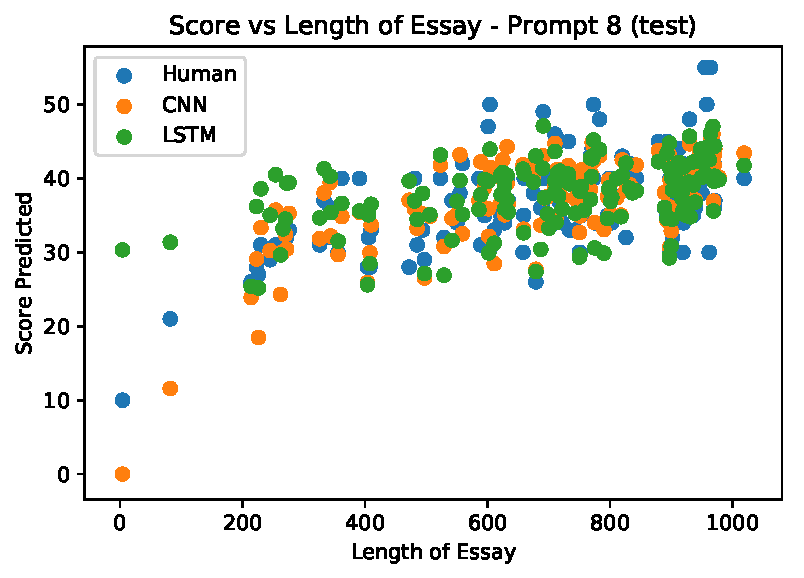
\includegraphics[width=\textwidth,ext=pdf]{{../../plots/score_vs_len_8_test}.pdf}
  \end{subfigure}
  \caption{Distribution of Length of essay and associated score in the test dataset \label{fig:length_plot}}        
\end{figure*}

\begin{table}[]
  \centering
  \resizebox{0.5\textwidth}{!}{%
  \begin{tabular}{|c|c|c|c|}
  \hline
  \textbf{Prompt} & \textbf{Essays Tested} & \multicolumn{2}{c|}{\textbf{\% Increase}} \\ \hline
  \textbf{} & \textbf{} & \textbf{Neural} & \textbf{Non-Neural} \\ \hline
  1 & 37 & \textbf{72.785} & \textbf{37.240} \\ \hline
  2 & 45 & 53.428 & \textbf{33.843} \\ \hline
  3 & 93 & \textbf{137.284} & \textbf{56.061} \\ \hline
  4 & 85 & \textbf{235.539} & \textbf{44.515} \\ \hline
  5 & 70 & \textbf{145.933} & 78.571 \\ \hline
  6 & 72 & \textbf{119.254} & 161.905 \\ \hline
  7 & 53 & 40.181 & \textbf{14.659} \\ \hline
  8 & 23 & 0.279 & \textbf{4.141} \\ \hline
  \end{tabular}%
  }
  \caption{Effect of Length}
  \label{length}
  \end{table}


\subsection{Effect of Spelling Mistakes}
We tried to analyze the effect of the spelling mistakes on the prediction of the models. We randomly chose 20\% of the words of the essay and then did a random shuffle of the characters to generate words with wrong spellings. We had a set of predicted scores for the essays with correct spellings and a new set of predicted scores for essays with wrong spellings. We calculated QWK between these two sets of scores. \cref{spell_word_sentence} shows that for the neural model, the QWK is close to 1 for most prompts whereas it is very close to 0 for non-neural model. Thus, for the neural model there is no disagreement between the scores predicted for essays with correct spellings and essays with 20\% wrong spellings.

% \begin{table}[]
%   \centering
%   \resizebox{0.5\textwidth}{!}{%  
%   \begin{tabular}{|c|c|c|c|}
%   \hline
%   \textbf{Prompt} & \textbf{Essays Tested} & \textbf{QWK (Neural)} & \textbf{QWK (Non-Neural)} \\ \hline
%   1 & 357 & \textbf{0.944} & \textbf{0.027} \\ \hline
%   2 & 360 & 0.408 & \textbf{0.013} \\ \hline
%   3 & 345 & \textbf{0.901} & \textbf{0.163} \\ \hline
%   4 & 355 & \textbf{0.936} & \textbf{0.019} \\ \hline
%   5 & 361 & \textbf{0.930} & \textbf{0.027} \\ \hline
%   6 & 360 & 0.591 & \textbf{0.017} \\ \hline
%   7 & 314 & \textbf{0.871} & \textbf{0.081} \\ \hline
%   8 & 145 & \textbf{0.822} & \textbf{0.086} \\ \hline
%   \end{tabular}
%   }
%   \caption{Effect of Spelling Mistakes}
%   \label{spelling}
%   \end{table}

\subsection{Effect of Word Shuffle}
We tried to analyze the effect of the bad grammar on the prediction of the models. We randomly shuffled the positions of words in each sentence of the essay set. This resulted in an essay with terrible grammar, and thus should be scored low by any good AES system. We had a set of predicted scores for the essays with good grammar and a new set of predicted scores for essays with bad grammar and a lot of grammatical mistakes. We calculated QWK between these two sets of scores. \cref{spell_word_sentence} shows that for the neural model, the QWK is close to 1 for most prompts whereas it is significantly less than 1 for the non-neural model. Thus, for the neural model there is no disagreement between the scores predicted for essays with correct grammar and essays with bad grammar.

% \begin{table}[]
%   \centering
%   \resizebox{0.5\textwidth}{!}{%    
%   \begin{tabular}{|c|c|c|c|}
%   \hline
%   \textbf{Prompt} & \textbf{Essays Tested} & \textbf{QWK (Neural)} & \textbf{QWK (Non- Neural)} \\ \hline
%   1 & 357 & \textbf{0.940} & 0.991 \\ \hline
%   2 & 360 & 0.739 & \textbf{0.515} \\ \hline
%   3 & 345 & \textbf{0.893} & 0.709 \\ \hline
%   4 & 355 & \textbf{0.930} & \textbf{0.495} \\ \hline
%   5 & 361 & \textbf{0.913} & \textbf{0.251} \\ \hline
%   6 & 360 & \textbf{0.914} & \textbf{0.306} \\ \hline
%   7 & 314 & \textbf{0.944} & 0.962 \\ \hline
%   8 & 145 & \textbf{0.934} & 0.931 \\ \hline
%   \end{tabular}
%   }
%   \caption{Effect of Word Shuffle}
%   \label{word_shuffle}
%   \end{table}

\subsection{Effect of Sentence Shuffle}
  We tried to analyze the effect of the bad organization and flow of ideas on the prediction of the models. We randomly shuffled the sentences of the essay. This resulted in an essay with terrible organization and flow of ideas, and thus should be scored low by any good AES system. We had a set of predicted scores for the essays with good flow of ideas and a new set of predicted scores for essays with a poor organization. We calculated QWK between these two sets of scores. \cref{spell_word_sentence} shows that for both the the models, the QWK is close to 1 for most prompts. Thus, there is no disagreement between the scores predicted for essays with good organization and flow of ideas and essays without it for both the models.

% \begin{table}[]
%   \centering
%   \resizebox{0.5\textwidth}{!}{%
%   \begin{tabular}{|c|c|c|c|}
%   \hline
%   \textbf{Prompt} & \textbf{Essays Tested} & \textbf{QWK (Neural)} & \textbf{QWK (Non- Neural)} \\ \hline
%   1 & 357 & \textbf{0.919} & \textbf{1.000} \\ \hline
%   2 & 360 & \textbf{0.847} & \textbf{0.997} \\ \hline
%   3 & 345 & \textbf{0.906} & \textbf{0.995} \\ \hline
%   4 & 355 & \textbf{0.944} & \textbf{0.986} \\ \hline
%   5 & 361 & \textbf{0.903} & \textbf{0.998} \\ \hline
%   6 & 360 & \textbf{0.907} & \textbf{0.984} \\ \hline
%   7 & 314 & \textbf{0.977} & \textbf{0.998} \\ \hline
%   8 & 145 & \textbf{0.991} & \textbf{0.999} \\ \hline
%   \end{tabular}%
%   }
%   \caption{Effect of Sentence Shuffle}
%   \label{sentence_shuffle}
%   \end{table}

\begin{table*}[]
  \centering
  \resizebox{\textwidth}{!}{%
  \begin{tabular}{|c|c|c|c|c|c|c|c|}
  \hline
  \textbf{Prompt} & \textbf{Essays Tested} & \multicolumn{2}{c|}{\textbf{Spelling Mistakes}} & \multicolumn{2}{c|}{\textbf{Word Shuffle}} & \multicolumn{2}{c|}{\textbf{Sentence Shuffle}} \\ \hline
  \textbf{} & \textbf{} & \textbf{Neural} & \textbf{Non-Neural} & \textbf{Neural} & \textbf{Non-Neural} & \textbf{Neural} & \textbf{Non-Neural} \\ \hline
  1 & 357 & \textbf{0.944} & \textbf{0.027} & \textbf{0.940} & 0.991 & \textbf{0.919} & \textbf{1.000} \\ \hline
  2 & 360 & 0.408 & \textbf{0.013} & 0.739 & \textbf{0.515} & \textbf{0.847} & \textbf{0.997} \\ \hline
  3 & 345 & \textbf{0.901} & \textbf{0.163} & \textbf{0.893} & 0.709 & \textbf{0.906} & \textbf{0.995} \\ \hline
  4 & 355 & \textbf{0.936} & \textbf{0.019} & \textbf{0.930} & \textbf{0.495} & \textbf{0.944} & \textbf{0.986} \\ \hline
  5 & 361 & \textbf{0.930} & \textbf{0.027} & \textbf{0.913} & \textbf{0.251} & \textbf{0.903} & \textbf{0.998} \\ \hline
  6 & 360 & 0.591 & \textbf{0.017} & \textbf{0.914} & \textbf{0.306} & \textbf{0.907} & \textbf{0.984} \\ \hline
  7 & 314 & \textbf{0.871} & \textbf{0.081} & \textbf{0.944} & 0.962 & \textbf{0.977} & \textbf{0.998} \\ \hline
  8 & 145 & \textbf{0.822} & \textbf{0.086} & \textbf{0.934} & 0.931 & \textbf{0.991} & \textbf{0.999} \\ \hline
  \end{tabular}%
  }
  \caption{Effect of spelling mistakes, grammatical errors and poor organization in terms of QWK between old predicted scores and new predicted scores}
  \label{spell_word_sentence}
  \end{table*}


\section{Methods Proposed}

\subsection{Data Bootstrapping}
In the current dataset, most of the essays are reasonably good and hence the neural models are not able to learn that longer essays does not necessarily mean better scores. Also, it is not able to learn that spelling mistakes should reduce the overall score.
To overcome this problem we propose to augment the dataset with negative examples like adding longer essays with lower scores (by concatenating low score and small essays multiple times).  

\subsection{New Tokens}

Presently, the neural model used a special symbol of \textit{\textless UNK \textgreater} for out-of-vocabulary words. Thus words which have wrong spelling, were replaced with the embedding of \textit{\textless UNK \textgreater}. We added a new symbol \textit{\textless MISSPELL \textgreater}. We checked if word has correct spelling using a corpus of 200,000+ words and if it had a wrong spelling, it was replaced with the symbol \textit{\textless MISSPELL \textgreater}. We analyzed the effects of spelling mistakes on this model, and the results are shown in \cref{misp_diff} and suggest that \textless MISSPELL \textgreater helps in assigning low scores to misspelled essays.

\begin{table}[]
  \centering
  % \resizebox{0.5\textwidth}{!}{%
  \begin{tabular}{|l|l|}
  \hline
  \textbf{Prompt} & \textbf{QWK} \\ \hline
  1 & 0.792 \\ \hline
  2 & \textbf{0.277} \\ \hline
  3 & 0.888 \\ \hline
  4 & 0.837 \\ \hline
  5 & 0.907 \\ \hline
  6 & 0.890 \\ \hline
  7 & \textbf{0.636} \\ \hline
  8 & \textbf{0.242} \\ \hline
  \end{tabular}
  % }
  \caption{Effect of adding \textless MISSPELL\textgreater token (measure as QWK score between old prediction and new prediction)}
  \label{misp_diff}
\end{table}

% \begin{table}[]
%   \centering
%   \resizebox{0.5\textwidth}{!}{%
%   \begin{tabular}{|l|l|l|l|}
%   \hline
%   \textbf{Prompt} & \textbf{Previous Score} & \textbf{New Score} & \textbf{\% Decrease} \\ \hline
%   1 & 0.647 & 0.588 & \textbf{26.16} \\ \hline
%   2 & 0.469 & 0.268 & \textbf{10.07} \\ \hline
%   3 & 0.590 & 0.606 & \textbf{43.72} \\ \hline
%   4 & 0.458 & 0.376 & \textbf{36.21} \\ \hline
%   5 & 0.603 & 0.567 & \textbf{33.80} \\ \hline
%   6 & 0.667 & 0.618 & \textbf{25.98} \\ \hline
%   7 & 0.532 & 0.418 & \textbf{25.39} \\ \hline
%   8 & 0.614 & 0.449 & \textbf{11.68} \\ \hline
%   \end{tabular}%
%   }
%   \caption{Scores of new model (with \textless MISSPELL\textgreater token) and old model on essays with $20\%$ misspelled words.}
%   \label{misp_diff}
%   \end{table}
  
  

% \acomment{Add table for QWK changes with spelling mistakes on this model.}

\subsection{Hierarchial LSTM}

The current SoTA neural model, used basic LSTM cell to encode the whole essay. Typically, an essay has a length of about 500 tokens, and it is very hard for a LSTM to remember this long sequence. We propose using an hierarchical LSTM network to mitigate the long history length and to model grammar and coherence better. We effectively run a LSTM over the words of each sentence and generate a vector representation of the sentence and then run a LSTM over the representations of the sentences learned in the previous layer to generate a representation of the essay.\\ 
We were not able to get satisfactory results with this approach (shown in \cref{hlstm}). One of the possible explanations for this is that the dataset size is too small for hierarchical LSTM to learn the grammar.
% \acomment{Add table for QWK changes with word and sentence shuffle mistakes on this model.}


\begin{table}[]
  \centering
  \begin{tabular}{|l|l|}
  \hline
  \textbf{Prompt} & \textbf{QWK} \\ \hline
  1 & 0.962 \\ \hline
  2 & 0.915 \\ \hline
  3 & 0.912 \\ \hline
  4 & 0.966 \\ \hline
  5 & 0.954 \\ \hline
  6 & 0.934 \\ \hline
  7 & 0.976 \\ \hline
  8 & 0.970 \\ \hline
  \end{tabular}
  \caption{Effect of sentence shuffle (agreement between LSTM and Hierarchical LSTM using QWK metric)}
  \label{hlstm}
\end{table}


\section{Conclusions}
In this paper we have analyzed the behavior of neural model for automated essay scoring on various practical scenarios. We performed various experiments for effect of length, grammar, spelling, organization and found that neural models perform very poorly in these qualitative metrics even while giving state of art performance on the quantitative benchmarks. This shows that the problem of automated essay scoring is far from being solved and getting human level performance on benchmarks is not the solution. This also shows that the current benchmarks are not sufficient for evaluation and thus the need of better metrics. We have also suggested some solutions to problems like length-score correlation, misspelled words which seem to provide some robustness to above problems.


\bibliography{paper}
\bibliographystyle{acl_natbib}

\end{document}
